
\newcolumntype{L}[1]{>{\raggedright\let\newline\\\arraybackslash\hspace{0pt}}m{#1}}
\newcolumntype{C}[1]{>{\centering\let\newline\\\arraybackslash\hspace{0pt}}m{#1}}
\newcolumntype{R}[1]{>{\raggedleft\let\newline\\\arraybackslash\hspace{0pt}}m{#1}}



\section{Genomic variation and protein mutations}

The human genome carries the genetic information of a person. From individual to individual, there can be a certain degree of variation in the genome, and this variation can have many consequences. Often, the variation carries with it no real functional consequence. Sometimes, the variation can be beneficial, while at other times it can be highly harmful and associated with disease.

One type of variation is single nucleotide polymorphisms, SNPs. Here, a nucleotide at a certain position in the genome is exchanged for another nucleotide. SNPs can have widely varying effects depending on where in the genome they occur. If they occur in coding regions of the genome, they can be classified into synonymous substitutions and non-synonymous substitutions. Synonymous substitutions are those substitutions that result in a codon still coding for the same amino acid, while non-synonymous substitutions cause an amino acid change in the final protein product of the coding region.\cite{gonzales2002synonymous} Through population scale sequencing, it has been estimated that individuals, when compared to a reference genome, carry around 10 000 to 11 000 non-synonymous substitutions, and 10 000 to 12 000 synonymous substitutions.\cite{10002010map} Mutations occurring in the coding regions of the genome have been found to more often be associated with disease, compared to those occurring in non-coding regions.\cite{niroula2015pon}

An amino acid substitution can have several effects on a protein. It can affect the way the protein interacts with other proteins, how it folds, as well as how it is expressed and where it is localized in the cell.\cite{reva2011predicting} These factors and others, can also cause the protein to gain a new, different function than that of its original one, or lose its function.\cite{reva2011predicting}

Mutations with experimentally verified effects can be found in literature and databases. Detailed data connecting a certain mutation and the phenotypes it gives rise to can often be found in databases specifically dedicated for the study of a certain gene or disease: locus-specific databases (LSDBs).\cite{giardine2007phencode} Efforts exist to systematically collect and organize such data into larger, wide-spanning databases. Several repositories collect large amounts of annotated variants, such as the Human Gene Mutation Database (HGMD)\cite{stenson2009human} and the Single Nucleotide Polymorphism Database (dbSNP)\cite{sherry2001dbsnp}. The database VariBench\cite{nair2013varibench} collects and organizes variants from databases such as dbSNP into benchmark datasets, containing both positive and negative samples (i.e. variants having a certain effect and variants not having an effect). It contains datasets related to protein tolerance (whether variants are benign or not), protein stability, mismatch repair gene variation, protein mutations affecting transcription factor binding, as well as splice site variation.\cite{nair2013varibench} These datasets are useful for developing and assessing prediction tools intended for use in these domains. The sizes of these datasets vary, but the largest of these contains up to 19 000 pathogenic non-synonymous SNPs and 21 000 neutral non-synonymous SNPs.

\section{Predicting the effect of mutations}

\subsection{Variant effect predictors}

For predicting the effect of non-synonymous SNPs leading to protein mutations, a number of predictive tools have been developed. The meta-database OMICtools\cite{henry2014omictools} lists over 130 variant effect prediction tools, many of them made for predicting effects of amino acid substitutions. A collection of several such tools can be seen in Table \ref{table:predictors} on page \pageref{table:predictors}. The table describes tools in terms of what kinds of features in the input data the classifier looks at, what type of classifier the tool uses, what data the classifier is trained on if it is a machine learning approach, as well as general notes on the tool.

Some tools are specialized for certain types of variants, such as VEST\cite{carter2013identifying} for Mendelian disease mutations or PON-MMR2\cite{niroula2015classification} for variants in mismatch repair proteins.

Many of these tools employ some form of machine learning to train a predictor on a certain dataset, which then allows the predictor to generate a prediction on a novel mutation, given some input data. Others develop some form of rule or mathematical operation to calculate a score, which is then used to classify a variant. 

The performance of available predictors differs somewhat depending on what dataset they have been trained and tested on. Proper comparison of the performance of available predictors is made somewhat complicated since many have not been trained and tested on standard benchmark datasets. If such predictors are then evaluated on a standard test dataset, their performance can be biased due to overlap between datasets. Evaluations carried out using fully disjoint datasets found that the performance measures of most tools greatly decreased from their reported performance.\cite{grimm2015evaluation} Some bias is also introduced at a protein level, if variants from the same protein are present in training and testing datasets.\cite{grimm2015evaluation} However, some of the best performing predictors have taken care to avoid any such data circularity, and report classification accuracy up to 77\% with a Matthews correlation coefficient (MCC) of 0.53\cite{niroula2016variation} when classifying variants into pathogenic and neutral.


\subsection{Sequence information and features}

What most predictors have in common, especially those with good performance, is that they utilize information obtained from a multiple sequence alignment (MSA) of homologous protein sequences.\cite{miosge2015comparison} A homologous sequence (in terms of DNA or amino acids), is a sequence that has a statistically significant similarity to some reference sequence, which indicates common ancestry between the sequences.\cite{pearson2013introduction} Homologous sequences can further be divided into paralogs and orthologs, where paralogs arise from duplication of a gene within a genome, and orthologs arise from speciation events. While many variant effect predictors include all homologous sequences, certain predictive tools such as SNPdryad\cite{wong2014snpdryad} find that excluding paralogous sequences and only including orthologuous sequences in an MSA can improve classification accuracy.

Homologous sequences can be found by comparing a query sequence against a large database of other sequences, and evaluating similarity through some scoring scheme. One of the most common ways of doing this is by using BLAST\cite{altschul1990basic}, but can also more recently be done by using hidden Markov model (HMM) based approaches with programs like HMMER.\cite{eddy2009new}

The MSA built from homologous sequences can be used to calculate statistics indicating evolutionary conservation. For example, an MSA of homologous protein sequences can be used to infer how important a certain residue at a certain position is for maintaining function and structure of a protein.\cite{valdar2002scoring} An example of an MSA can be seen in Figure \ref{fig:msa}. If some position in an alignment of many similar proteins always seems to contain a certain amino acid, it is likely that the amino acid at that position is important for the protein function in some way. Scoring such conservation can be done in many different ways, but is often done by calculating some version of an entropy score, such as Shannon's entropy for a column in the MSA\cite{valdar2002scoring}:

\begin{equation}
S = -\sum_{i}^{K} p_i \log_2 p_i
\end{equation}

where $p_i$ is the fractional frequency of an amino acid of type \textit{i} out of \textit{K} types.

\begin{figure}
  \centering
  \hspace*{-0.8in}
  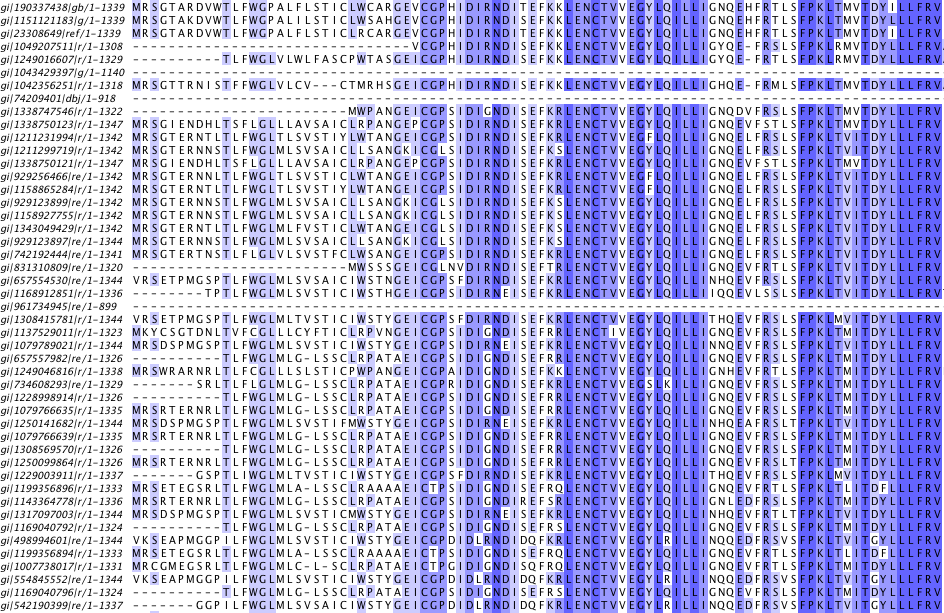
\includegraphics[scale=0.5]
    {msa_example_edited.png}
  \centering
  \caption{ MSA of protein sequences. Blue columns indicate more conserved positions. }
  \label{fig:msa}
\end{figure}


Certain predictors also use information about the structure of the protein of interest. This information can for instance determine if an amino acid substitution occurs in the hydrophobic protein core, or if it has an effect on electrostatic interactions or other interactions.\cite{adzhubei2013predicting} Other predictors include information about the physical and chemical properties of the amino acids involved in the mutation, and around the mutation site.\cite{niroula2017predicting}

\clearpage
\begin{center}
\setlength\LTleft{-1.2in}
%\setlength\LTright{-1in}
\begin{small}
\begin{longtable}{| l | L{4cm} | L{2cm} | L{3cm} | L{5cm} |}
\caption{Variant effect predictors able to handle amino acid substitutions.\\Abbreviations: AA (amino acid), RF (random forest), GO (gene ontology), MSA (multiple sequence alignment), SVM (support vector machine)}
\label{table:predictors}
\endfirsthead
\endhead
\hline
Predictor & Features & Classifier type & Training dataset & Notes \\ \hline
PON-P2 & Evolutionary conservation, physical and biochemical properties of AAs, GO annotations & RF & VariBench PON-P2 & Classifies into pathogenic/neutral/unknown.  \\ \hline
PON-MMR2 & Similar to PON-P2 & RF & VariBench PON-MMR & Specialized for mismatch repair proteins. Classifies into pathogenic/neutral. \\ \hline
PON-PS & Similar to PON-P2 & RF & VariBench PON-PS & Predicts severity of AA substitutions. Classifies into severe and nonsevere. \\ \hline
MutationAssessor & Functional impact score based on evolutionary information & Score threshold &  N/A & Specialized for cancer genomics. \\ \hline
SIFT & Scaled probabilities of AAs in positions in MSA & Score threshold & N/A & MSA created from homologs found with BLAST. Classifies into tolerated/deleterious. \\ \hline
PolyPhen-2 & Features from sequence annotations, MSA, 3D structures & Naive Bayes & HumDiv / HumVar (compiled from variants in UniProtKB) & Calculates the posterior probability that a mutation is damaging. \\ \hline
PROVEAN & Differences in E-value from BLAST & Score threshold & N/A & Uses delta score (function of change in alignment score because of a substitution). Can handle several simultaneous substitutions in a protein. \\ \hline
MutationTaster2 & Regulatory features from Ensembl, evolutionary conservation scores of nucleotides & Bayes classifier  & Polymorphisms from 1000G, mutations from HGMD & Starts from DNA sequence; can also handle synonymous substitutions. \\ \hline
VEST & Features from SNVBox & RF & Mutations from HGMD and variants from the Exome Sequencing Project & Specialized for mendelian disease mutations. \\ \hline
CADD & Annotations from Ensembl VEP and scores from other programs & SVM & Simulated variants and variants from ClinVar & Combines annotations and scores from many different programs. \\ \hline
FATHMM & AA probabilities in a HMM & Score threshold & N/A & The HMM is constructed from an MSA obtained with JackHMMER. \\ \hline
PMUT & Features from internal databases, structural features, features from MSA & Shallow neural network & Not specified & Outputs a pathogenicity index ranging from 0 to 1. \\ \hline
PantherPSEP & Evolutionary score from MSA & Score threshold & HumVar & Obtains alignments from PANTHER database. \\ \hline
MAPP & Score based on MSA and physiochemical properties of AAs & Score threshold & N/A & Classifies into neutral/moderately deleterious/strongly deleterious. \\ \hline
Align-GVGD & Grantham variation and difference of a position in MSA & Score threshold & N/A & Grantham analysis is based on physiochemical characteristics of amino acids. \\ \hline
DANN & Same as CADD & Neural network & Same as CADD & Network structure:
input layer, sigmoid output layer, three 1000-node tanh hidden layers. \\ \hline
Condel & Combines predictions from Logre, MAPP, MutationAssessor, PolyPhen-2, SIFT & N/A & N/A & Consensus tool. \\ \hline
SNPdryad & Features from MSA of orthologous proteins, physiochemical properties of AAs & RF & HumDiv and HumVar & Found that excluding paralogs leads to better performance. \\ \hline
SNAP2 & Wide range of amino acid properties, explicit sequence, PSIC profiles, various structural properties, residue flexibility, various annotations, contact potentials & 10 different shallow neural networks  & Variants from PMD, SWISS-PROT, OMIM, HumVar & Uses a very wide range of features. Classifies into effect/neutral. \\ \hline
\end{longtable}
\end{small}
\end{center}
\clearpage

\section{Machine learning}

\subsection{Conventional methods}
As can be seen in Table \ref{table:predictors}, the vast majority of tools based on machine learning are conventional machine learning approaches. In this approach, feature engineering is done on the input data to extract feature vectors which are then fed into some classifier. Some common classifier types for variant effect prediction are Random Forest (RF) classifiers, Support Vector Machine (SVM) classifiers, and some more simple probabilistic classifiers such as the Naive Bayes classifier.

\subsection{Feature engineering and selection}
The feature engineering in many of the tools can be quite involved. Often, it requires collecting data from many different sources and running what can sometimes be computationally expensive steps. For example, a very informative feature is codon-level selective pressure\cite{niroula2015classification}, but it requires collecting a protein's corresponding cDNA sequence, aligning codons, and computing on the alignment. This computational expense can be alleviated somewhat though, by using pre-computed feature vectors when making predictions.

When having a large feature set, feature selection is also a step that has to be done for most machine learning approaches. This can involve methods ranging from simple filter methods to more computationally expensive wrapper methods such as forward feature selection.

\section{Deep learning}

\subsection{Problem domains}

Some of the more recent tools in Table \ref{table:predictors} are based on neural networks, some with several hidden layers. As of yet, though, they are mostly shallow densely connected feedforward networks using similar (or the same in one case) features as more conventional tools. One advantage of deep learning approaches is that it allows for an end-to-end feature extraction and classification model based on lower level representations of input data.

Deep learning methods have recently shown promise in many other applications of predicting properties of proteins. Deep learning shows success in protein contact prediction\cite{skwark2014improved}, and for assessing protein model quality, a Multilayer Perceptron (MLP) achieves state-of-the-art results.\cite{uziela2017proq3d} 

More complex architectures can be found in other problem domains. DeepCNF\cite{wang2016protein} utilizes a deep convolutional neural network (CNN) combined with conditional neural fields\cite{peng2009conditional} to predict the secondary structure of a protein. It does this using only a sparsely encoded amino acid sequence and a position specific scoring matrix (PSSM) obtained from an MSA as input.

For some problem domains, an encoding of only the protein sequence itself is used as input to deep models. This has been used to predict protein function in a model using a Recurrent Neural Network (RNN), containing long-short-term-memory (LSTM) units.\cite{liu2017deep} Another model predicts enzyme function with a network combining both CNN and RNN components.\cite{li2017deepre} Using only a sequence might not be enough information input for a problem heavily dependent on evolutionary information, however.

\subsection{Multilayer perceptrons}

One of the most simple types of deep neural networks are MLPs. Some of the predictors in Table \ref{table:predictors} belong to this class of network. MLPs consist of an input layer, an output layer, and a number of hidden layers in between. Each layer consists of a number of neurons, or nodes. Nodes are connected in a feedforward fashion with a weight parameter for each connection. Each node computes an output from an activation function involving its connections and their weights, as well as a bias. This computation can be described for some activation function \textit{f}, weight vector \textbf{w}, input vector \textbf{x} and bias \textit{b} as follows:

\begin{equation}
y = f(\mathbf{w}^T\mathbf{x} + b)
\end{equation}

Often used activation functions include the logistic sigmoid function

\begin{equation}
\sigma(x) = \frac{1}{1 + e^{-x}}  
\end{equation}

or the activation function used in a rectified linear unit (ReLU)

\begin{equation}
f(x) = \textrm{max}(0,x)  
\end{equation}

By stacking several layers of such nodes in a network, the network becomes capable of approximating non-linear functions. For a given set of input and output data, network parameters can be adjusted in a supervised fashion. This allows the network to capture relationships between input features and be used for classification problems. Network parameters are adjusted using some form of loss function such as the mean squared error (MSE) or the cross-entropy loss between network output and desired output, along with a gradient-based optimization algorithm. For computing the gradient on which to base a parameter update, back-propagation is used. For updating the parameters, several optimization algorithms exist such as stochastic gradient descent (SGD) or more recent variants thereof such as Adam.\cite{kingma2014adam}

\subsection{Convolutional networks}

Convolutional neural networks share some similarities to the multilayer perceptrons described above. It is a feedforward network, uses similar activations, and is trained in the manner described above. However, a convolutional network makes use of sparse connectivity by only connecting neurons in a hidden layer to a certain region of input, and sliding this region across the input space. Additionally, instead of using individual weights and biases for each neuron, neurons share parameters, defining a filter. A convolutional layer will then consist of a number of such filters. Typically, a convolutional network will also make use of so-called pooling layers applied on the feature maps created by convolutional layers, to create a more condensed version of these.
An example of a convolutional network can be seen in Figure \ref{fig:deepsf}, applied to protein sequence derived input.

\begin{figure}
  \centering
  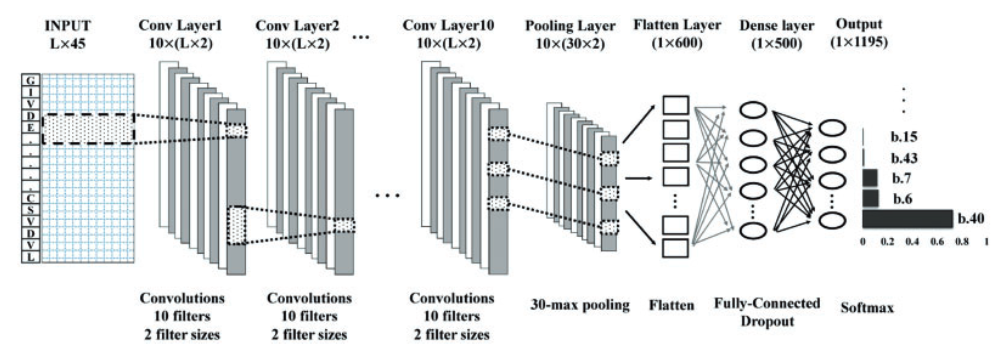
\includegraphics[scale=0.4]
    {DeepSF_model_2.png}
  \centering
  \caption{ 1D deep convolutional network used in DeepSF. Reproduced from Hou et al, 2017.\cite{hou2017deepsf} }
  \label{fig:deepsf}
\end{figure}

While not widely used for variant effect prediction problems, convolutional networks have shown remarkable success in other protein prediction domains. One state-of-the-art model for contact prediction\cite{wang2017accurate} uses residual neural network blocks with first 1-dimensional and then 2-dimensional convolutions, using MSA-derived features and some other protein features as input. The structure of the network allows it to handle proteins of varying length. Similar input features are used in another model combining six CNNs, also for contact prediction.\cite{adhikari2017dncon2} Other examples of 1-dimensional CNN models applied to protein sequences are Must-CNN, used for structural prediction\cite{lin2016must} and DeepSF, for mapping protein sequences to folds.\cite{hou2017deepsf} Going beyond those problems based on protein sequences, CNNs have been used to predict effects of non-coding variants in DNA sequences.\cite{zhou2015predicting}

A 1D convolutional layer can learn to recognize local patterns in a sequence, and these patterns can then be recognized at other locations in the sequence. 2D layers have such properties for local patches in a matrix. These local patterns are able to capture important relationships between, for example, amino acids in a sequence.





